\chapter{Convective mass transfer}

\section{Mass transfer with advection}

In a situation where the domain consists of species A and B and we are
interested in the flux of species A, there are following possible situations.

\begin{itemize}
\item Species B is not present / species A is very dilute in B and thus B can be
said to not take part in the diffusion process. In this situation, the flux is
given by Fick's first law.
\item Species B is present and takes part in the diffusion process.
Additionally, an assumption can be made that net flux of B is zero and species B
moves only to replace species A. This approach is called \textbf{stagnant layer}
approach.
\item Species B is present and the domain is not stagnant. In such a situation,
the influence of bulk velocity on the flux of both species be determined
separately.
\end{itemize}

The first case is simple as discussed in the previous section. For the second
case, we can proceed by assuming that the flux is one dimensional and the
velocity of the species A is $v$ which is same (but opposite in direction) for
species B. 

The total flux that takes advection into account can be
given as:

$$ \boxed{
 \vec{j_A} = -D_{AB}\vec{\nabla} \rho_A + \vec{u} \rho_A 
}$$

Where, $\vec{j_A}$ is the \textbf{net} flux of species A taking the advection
into account.

\section{Mass transfer with advection}

In a situation where the domain consists of species A and B and we are
interested in the flux of species A, there are following possible situations.

\begin{itemize}
\item Species B is not present / species A is very dilute in B and thus B can be
said to not take part in the diffusion process. In this situation, the flux is
given by Fick's first law.
\item Species B is present and takes part in the diffusion process.
Additionally, an assumption can be made that net flux of B is zero and species B
moves only to replace species A. This approach is called \textbf{stagnant layer}
approach.
\item Species B is present and the domain is not stagnant. In such a situation,
the influence of bulk velocity on the flux of both species be determined
separately.
\end{itemize}

The first case is simple as discussed in the previous section. For the second
case, we can proceed by assuming that the flux is one dimensional and the
velocity of the species A is $v$ which is same (but opposite in direction) for
species B. 

The total flux that takes advection into account can be
given as:

$$ \boxed{
 \vec{j_A} = -D_{AB}\vec{\nabla} \rho_A + \vec{u} \rho_A 
}$$

Where, $\vec{j_A}$ is the \textbf{net} flux of species A taking the advection
into account.

\subsection{Mass transfer coefficient}

In many situations, it may be favourable to define a mass transfer coefficient
akin to heat transfer coefficient such that one can experimentally or otherwise
determine it. The definition is as given below:

$$ j_A = k_A \left( C_A - C_{A0} \right) $$

If the units of $C_A$, as used commonly, are mass/vol then the units of $k_A$
are same as those of velocity. Once the mass transfer coefficient is known, flux
can be determined using the above equation. In situations such as solid state
diffusion, $k_A$ can be determined by evaluating the slope of the species
distribution (say, error function) itself.

Eg., for transient diffusion in solid / quiescent liquid whose bulk composition
is $C_{A0}$ and is in contact with atmosphere with zero concentration of species
A as illustrated in the figure, we can write the following flux balance.

\begin{figure}[h]
\begin{center}
\framebox{
 \includegraphics[scale=0.7]{images/c21-surfrenewfig.ps}
}
\end{center}
\caption{Surface Renewal Approach}
\label{surfrenew}
\end{figure}

Writing the composition distribution for species A in the domain,

$$ { C_A \over C_{A0} } = \text{erf} \left({x \over 2\sqrt{D_{AB}t}}\right)$$

Evaluating the flux at the interface at time t,

$$ k_{A,t} \left( C_{A0} - 0 \right) = j_A = | - \left. D_{AB} {\partial C_A
\over \partial x} \right|_{x \rightarrow 0} | = D_{AB} C_{A0} \left. {2 \over
\sqrt{\pi}} e^{-\left({x \over 2\sqrt{D_{AB}t}}\right)^2} {1 \over \sqrt{D_{AB}
t}} \right|_{x \rightarrow 0}$$

$$ k_{A,t} = 2 \sqrt{D_{AB} \over \pi t} $$

This is the instantaneous mass transfer coefficient. The time averaged
coefficient will be obtained by averaging the coefficient over the time interval
$t=0$ to $t=t$.

$$ \boxed{
k_A = \sqrt{D_{AB} \over \pi t} 
}$$

In case of a steadily falling (along $z$ axis) film of liquid, the quantity $z
\over u_{z,\text{max}}$ plays the role of time. The $z$ averaged mass transfer
coefficient will then be given as

$$ \boxed{
k_A = \sqrt{D_{AB} u_{z,\text{max}} \over \pi z} 
}$$

\subsection{Film Theory}

\begin{figure}[h]
\begin{center}
\framebox{
 \includegraphics[scale=0.7]{images/c21-filmtheoryfig.ps}
}
\end{center}
\caption{Film Theory}
\label{filmtheory}
\end{figure}

Mass transfer coefficient $h_m$ can be estimated as follows.

$$ h_m \left( C_A^s - C_A^\infty \right) = \left| j_A \right| $$

$$ j_A = \left| -D {\partial C_A \over \partial x} \right|_{x \rightarrow 0} = {D \left( C_A^s - C_A^\infty \right) \over \delta} $$

\begin{equation}
\boxed{
	h_m = {D \over \delta}
}
\end{equation}

\subsection{Penetration Theory}

\begin{figure}[h]
\begin{center}
\framebox{
 \includegraphics[scale=0.7]{images/c21-penetrationtheoryfig.ps}
}
\end{center}
\caption{Schematic of penetration theory. Here, $t_2 > t_1$.}
\label{penetrationtheory}
\end{figure}

Mass transfer coefficient $h_m$ can be estimated as follows.

$$ h_m \left( C_A^s - C_A^\infty \right) = \left| j_A \right| $$

$$ j_A = \left| -D {\partial C_A \over \partial x} \right|_{x \rightarrow 0} $$

$$ { C_A - C_A^\infty \over \left( C_A^s - C_A^\infty \right) } =  \text{erf} \left( {x \over 2 \sqrt{D t} } \right) $$

$$ j_A = D \left( C_A^s - C_A^\infty \right) {2 \over \sqrt{\pi}} {1 \over 2 \sqrt{Dt} } $$

\begin{equation}
\boxed{
	h_m = \sqrt {D \over \pi t}
}
\end{equation}


\subsection{Surface Renewal Theory}

\begin{figure}[h]
\begin{center}
\framebox{
 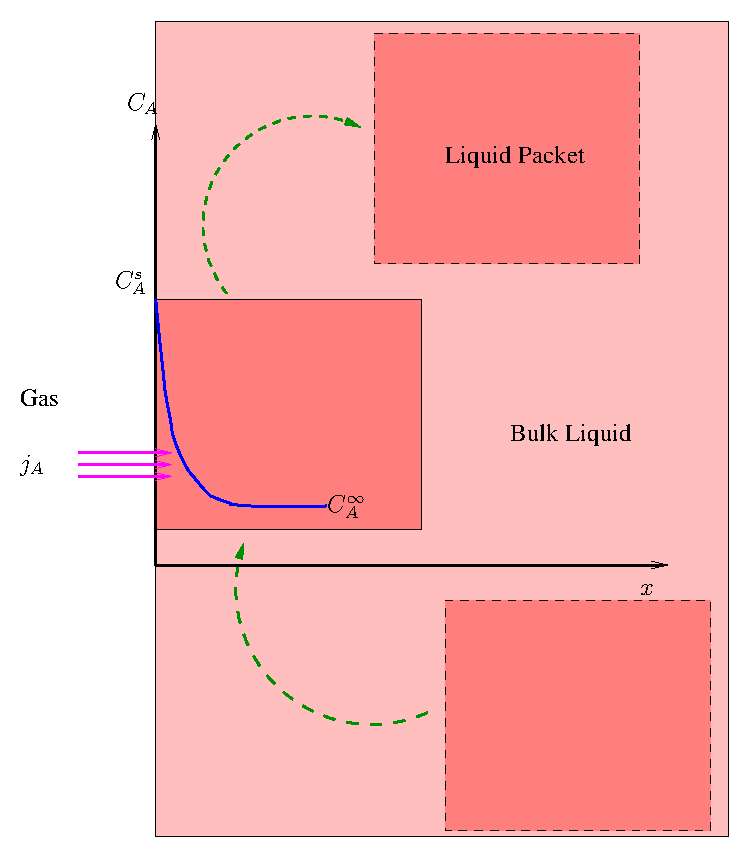
\includegraphics[scale=0.7]{images/c21-surfacerenewaltheoryfig.ps}
}
\end{center}
\caption{Schematic of surface renewal theory.}
\label{surfacerenewaltheory}
\end{figure}

Let $\tau$ be the time scale of the process that brings a pocket of fresh liquid to the surface (agitation frequency or residence time of a bubble etc. The probability of a liquid packet uniformly mixed with a concentration of species A of $C_A^\infty$ is given as $ {1/\tau}\, e^{-t\over\tau} $

We can see that the following identity holds for the probability distribution.

$$ \int_{0}^{\infty}{ {1\over \tau} e^{-t\over \tau} dt} = 1 $$

The instantaneous heat transfer coefficient for diffusional heat flux at time $t$ is given by the following.

$$ h_m\left( t \right) = \sqrt{D \over \pi t} $$

The averaged mass transfer coefficient taking the probability of the liquid packet being available at the surface into account,

$$ \bar{h}_m = \int_{0}^{\infty}{ \sqrt{D \over \pi t} {1 \over \tau} e^{-t\over\tau} dt} = \sqrt{D \over \tau}$$


The mass transfer coefficient can be given as follows.

\begin{equation}
\boxed{
	\bar{h}_m = \sqrt {D \over \tau}
}
\end{equation}


\subsection{Sherwood number}

Like the heat transfer coefficient is obtained in non-dimensionalized form by
encapsulating it with the thermal conductivity and characteristic length scale
as Nusselt number, mass transfer coefficient is also obtained in
non-dimensionalized form by encapsulating it with the solute diffusivity and
characteristic length scale as Sherwood number.

$$ Sh = {k_A L_c \over D_{AB}}$$

Sherwood number is determined experimentally as a function of Reynold's number
and Schmidt number to obtain correlations for advection aided mass transfer.

$$Sc = {\nu \over D_{AB}}$$

Examples:

Mass transfer from a sphere:

$$Sh_D  = 2 + C Re_D^m Sc^{1 \over 3}$$

The constants $C$ and $m$ depend on the range of $Re$ and $Sc$.

Mass transfer from a plate of length L (for $Re < 2 \times 10^5$):

$$ Sh_L = 0.664 Re_L^{0.5} Sc^{1 \over 3}$$ 


\section{Exercises}

\begin{enumerate}
\item Suppose that a hollow cylinder of nickel is used to measure the diffusion coefficient of hydrogen through this material. The cylinder has an outer diameter of \SI{2}{\milli\meter} and an inner diameter of \SI{1}{\milli\meter}. A CH$_4$/H$_2$ mixture is passed through the base of the cylinder which fixes the hydrogen concentration on the inner wall as 0.01 wt\%. Hydrogen diffusing through the cylinder is evacuated so that the hydrogen concentration on the outerwall is effectively zero. If hydrogen is collected under steady-state conditions at a rate of \SI{1.1e-11}{\mole\per\second} from the cylinder, \SI{2}{\centi\meter} long, held at \SI{200}{\celsius}, what is the diffusion coefficient? Take the density of nickel as \SI{8790}{\kilo\gram\per\meter\cubed}. {\bf Ans:} \SI{1.38e-11}{\meter\squared\per\second}

\item A dopant B is sent into a block of metal A of square cross-section. The flux of B is given as a constant. Making suitable assumptions, determine the concentration of B as function of distance from the surface of the bar if it is held at a high temperature for a long duration. What would be a good measure of depth of dopant penetration?

\item Nickel alloys are used in gas turbine engines at temperatures in excess of \SI{1000}{\celsius}. If pure nickel is exposed to air at \SI{1000}{\celsius} it will develop a coherent oxide scale. Determine how thick the oxide scale will be after 1, 10, 100 hours. Diffusivity is \SI{2.5e-15}{\meter\squared\per\second}. \\
Tips: Assume film theory is applicable. It is known that NiO becomes metal deficient to become Ni$_{1-x}$O as the oxygen potential is increased. In equilibrium with air at \SI{1000}{\celsius}, $x=3\times10^{-3}$.  {\bf Ans:} 232 nm, 735 nm and 2.32 $\mu$m.
{\bf Check if more data is needed}

\item Develop an expression for the drop in pressure of a steel cylinder that contains hydrogen  gas. 

\item For an iron melt at \SI{1600}{\celsius}, determine the maximum rate of iron evaporation and the corresponding thickness of the iron vapour layer. Assume an argon / oxygen atmosphere with a total pressure of \SI{1}{\bar}. Partial pressure of iron is \SI{7.5e-5}{\bar}, diffusivity of iron in argon is \SI{5.6e-4}{\meter\squared\per\second}. {\bf Ans:} \SI{0.1}{\mol\per\meter\squared\per\second}, \SI{2.7}{\micro\meter}.


\item A thin sheet of iron at \SI{800}{\celsius} is subjected to different gaseous atmospheres on both of its surfaces such that the composition of one face is 4 at\% carbon and the other is at 0 at\% carbon. At steady state, make a plot of the composition profile in the sample indicating clearly compositions and respective distances. The thickness is \SI{1}{\milli\meter} and density changes during experiment may be neglected. At \SI{800}{\celsius} it is known that the diffusion coefficient of carbon in iron is given by \SI{e-6}{\centi\meter\squared\per\second} in ferrite and \SI{e-8}{\centi\meter\squared\per\second} in austenite. {\bf Ans:} $\alpha$ is \SI{0.845}{\milli\meter} thick, interface is with 0.096 and 2.238 at\% carbon, respectively.

\item A thin layer of gold is plated on to the end of a nickel bar. The bar is annealed at \SI{900}{\celsius} for \SI{10}{\hour}. At this temperature, the interdiffusion coefficient of gold in nickel is \SI{1e-11}{\centi\meter\squared\per\second}. After this treatment, the concentration of gold at a distance of \SI{0.05}{\centi\meter} from the end is 0.1 at fraction of gold. At what distance is the atom fraction of gold equal to 0.01? {\bf Ans:} \SI{5.0033}{\centi\meter}

\item An electronic circuit plate is being protected from corrosion due to atmospheric moisture by a two layer coating of polymers. Assume a small gap between the two layers of polymers. If the two layers have different reaction constants for equilibrium with water vapour and different diffusivities, model how to determine the flux of moisture towards the circuit plate. Assume that the RH in the atmosphere is known. Draw schematically the variation of concentration of water vapour in the polymer layers as function of distance.

\item Silicon can be grown by CVD of silane. Given a system in which silicon grows from the bottom of an inert crucible with the top flushed by pure silane at 1 atm, predict the growth rate of silicon. Assume that the gas/silicon interface equilibrium is established according to the following reaction. 
$$ \text{SiH}_{4\text{(g)}} = \text{Si}_{\text{(s)}} + 2\text{H}_{2\text{(g)}} $$ 
The equilibrium constant is given by $K = 10^{-4} \, \text{atm}$. The diffusion coefficient in the gas at the reaction temperature \SI{700}{\kelvin} can be taken as \SI{1}{\centi\meter\squared\per\second}. {\bf Ans:} \SI{108}{\micro\meter\per\second}

\item When ceramic oxides are used to contain molten metals, they can dissolve and add undesirable impurities to the melt. This is especially true when melting is done under vacuum. For examples, magnesium oxide decomposes slowly according to the following equation.
$$ \text{MgO}_{\text{(s)}} = \text{[Mg]} + \text{[O]} $$
The square brackets indicate dissolution in the melt. The equilibrium constant for this reaction is $K = C_{Mg} C_O = 10^{-6}$ where $C_{Mg}$ and $C_O$ are concentrations in \SI{}{\mole\per\meter\cubed} of melt of Mg and O, respectively. For flow parallel to a \SI{3}{\meter} long plate of MgO, calculate the average mass transfer coefficient for Mg dissolving in the melt. Assume that $C_{Mg} = C_O$. For $x<0$, $C_{Mg}=0$ in the melt and V = \SI{3}{\meter\per\second}. What is the average flux of MgO dissolving in the melt? {\bf Ans:} \SI{3.15e-4}{\meter\per\second}, \SI{3.15e-7}{\mole\per\meter\squared\per\second}.\\
Density of the melt is \SI{8000}{\kilo\gram\per\meter\cubed}, thermal conductivity is \SI{50}{\watt\per\meter\per\kelvin}, heat capacity is \SI{840}{\joule\per\kilo\gram\per\kelvin}, viscosity is \SI{1.24e-3}{\newton\second\per\meter\squared} and diffusivities of both the species are \SI{5e-9}{\meter\squared\per\second}. For turbulent conditions, take $$ Sh_L = 0.037 Re_L^{0.8} Sc^{1/3}$$. 
\end{enumerate}
